\subsection{Example: let's rip off tetris}
\label{sec:casestudy}
Recall our exploration of tetriminos from Chapter~\ref{sec:simpleloop}. We
know enough now to turn this into an actual game of terminal Tetris\footnote{There
are a great many distinct Tetris implementations. We'll aim for loose
conformance to the NES version as published by Nintendo of America, because
I'm old. See \url{https://tetris.wiki/Tetris_(NES,_Nintendo)}. I'm not going
to obsess over details, though.}. Our implementation is fewer than 200 lines
total, yet it unites most of the techniques introduced in the past few
chapters. For fun, we'll do this in \CC\footnote{LOL how often does one hear
that said?}, using Marek Habersack's \CC wrappers (installed with Notcurses).

Our \texttt{main()} will parse command line options, set up a \texttt{Tetris}
object appropriately, and watch for input. The \texttt{Tetris} object provides
a thread function \texttt{Ticker} which moves the current piece down according
to timer events (calling \texttt{StuckPiece} to determine if the piece has been
placed, in which case a new piece enters the playing area), and the necessary
interface for the input loop:

\begin{denseitemize}
\item{\texttt{MoveLeft()} and \texttt{MoveRight()}
    (Listing~\ref{list:tetris-move}). These simply verify that the lateral
    move can be done, and then call \texttt{Plane::move()}.}
\item{\texttt{MoveDown()} (Listing~\ref{list:tetris-movedown}), which calls the same \texttt{StuckPiece()},}
\item{\texttt{Pause()}, and}
\item{\texttt{RotateCCw()} and \texttt{RotateCw()}, which verify that the rotation
      is possible, and then call \texttt{Plane::rotate\_cw()} or \texttt{Plane::rotate\_ccw()}.}
\end{denseitemize}

The general structure of our solution is thus:

\begin{denseitemize}
\item{A background is drawn onto the standard plane.}
\item{A new plane is created for the game area. Why make a new plane? Recall
    the beginning of Chapter~\ref{sec:planes}: \textit{we use a plane wherever we
    benefit from distinct state}. By keeping the game area on its own plane,
    we can trivially move it in response to terminal resizes, and likewise
    trivially test whether the current piece can move in a given direction.}
\item{Two tetrimino planes are created, one for the current piece, and one for
    the next piece. The current piece descends from the top of the game area.
    Upon reaching its final position, its plane is added to the game plane
    using \texttt{ncplane\_mergedown()}. The next piece is brought to the top
    of the game area, and the current piece is redrawn on its way to becoming
    the next piece.}
\item{We need no external state save the score and the order of pieces. The order
    of pieces is left up to the PRNG. We only need track the score and
    our four planes. The validity of a given movement can be checked entirely
    by reflection, using \texttt{ncplane\_at\_yx()}.}
\item{Our main thread loops on \texttt{Notcurses::getc()}, calling into the
    \texttt{Tetris} object. These calls will need to lock against the timer thread.}
\item{If \texttt{StuckPiece()} returns \texttt{true}, and the stuck piece
    is at the top of the playing area, the game is over.}
\end{denseitemize}

The playing area should not be visible while the game is paused, so whenever
the game is paused, we'll move the standard plane to the top of the z-axis. As
it is opaque and spans the visible area, this will hide the playing area. We'll
furthermore throw up a three-row plane centered on the screen; this plane will
contain a perimeter, and pulsing text reading ``Paused''. On an unpause event,
the attract plane is destroyed, and the standard plane moved back to the bottom
of the z-axis. Nothing else needs be touched, save inhibiting the operation
of \texttt{Ticker()}. This could be done any number of ways; we'll use a
condition variable plus a bit flag, checking it upon emerging from our timeout.

Our resize logic is pretty simple: on a resize event, after verifying that the
new geometry is large enough to play on (if not, we pause the game), we must
redraw the background, move the playing area to the new bottom center of the
visible area, and move the current piece to its same location relative to the
playing area. If the game is already paused when we resize, we ought
additionally recenter the attract plane\footnote{Imagine that we sized the playing area according to the
visible area. This would require resizing the game board upon a terminal
resize, a decidedly messier affair. It's \textit{doable}---\textgreek{ἢ τὰν ἢ ἐπὶ τᾶς}.}.

\pagebreak

\begin{listing}[!htb]
\inputminted[]{C}{code-tetris/gravity.h}
\inputminted[]{C}{code-tetris/stain.h}
\caption{Tetris helpers \texttt{Gravity()} and \texttt{StainBoard()}.}
\label{list:tetris-gravity}
\end{listing}

Let's do some boring groundwork first. We'll need the official constants for
``gravity'', the level-dependent rate at which pieces fall
(Listing~\ref{list:tetris-gravity}). We can implement this as a
\texttt{constexpr} function, not that it's likely to be of any real
advantage (especially since we only call \texttt{Gravity()} upon level changes).

\begin{listing}[!htb]
\inputminted[]{C}{code-tetris/clear.h}
\caption{\texttt{Tetris::LineClear()}.}
\label{list:tetris-lineclear}
\end{listing}

We'll need a function to tell us whether a line has been cleared
(Listing~\ref{list:tetris-lineclear}). We could track the state of the board
ourselves as a simple boolean matrix, but why bother when we can just ask the
source? Reflecting on a Notcurses plane is good practice of the
DRY\footnote{Don't Repeat Yourself.} principle. These aren't system calls,
just cheap indexed lookups into a framebuffer. It's unlikely that you can
do significantly better with your own implementation, so why bother? Let
Notcurses handle the state for you.

\begin{listing}[!htb]
\inputminted[]{C}{code-tetris/background.h}
\caption{Drawing the background and the gameplay plane.}
\label{list:tetris-background}
\end{listing}

Our background function (Listing~\ref{list:tetris-background}) just loads up
the provided image, stretched to fill the standard plane, blits it, and then
converts it to greyscale (so as not to be confused with actual playing pieces,
all of which are in color). The board is a double-lined box with the top
missing, and is its own plane. We also make a distinct plane for the score
and other textual info; this is useful as a last-ditch stopgap preventing
such text from spilling into the play area. Placing the board on its own
plane (as opposed to blitting it destructively onto the background) has two
major advantages: it simplifies responding to a terminal resize, and it allows
us to determine illegal moves via reflection on this plane.

\begin{listing}[!htb]
\inputminted[]{C}{code-tetris/stuck.h}
\caption{\texttt{Tetris::InvalidMove()}.}
\label{list:tetris-stuck}
\end{listing}

This brings us to \texttt{InvalidMove()} (Listing~\ref{list:tetris-stuck}).
All of our movement functions to come will need a means to test whether the
selected movement is legal, whether it's a lateral translation (\texttt{MoveLeft()}
and \texttt{MoveRight()}), a rotation (\texttt{RotateCw()} and \texttt{RotateCcw()}),
or falling towards the bottom (\texttt{MoveDown()}, called when the user presses
down and when the timer expires). Similarly to \texttt{LineClear()}, it's easiest
to leverage the Notcurses state. All five of these functions operate by speculatively
transforming the current piece, testing for overlap with the gameboard plane,
and pulling the piece back if there was an overlap.

\begin{listing}[!htb]
\inputminted[]{C}{code-tetris/movedown.h}
\caption{\texttt{Tetris::MoveDown()}.}
\label{list:tetris-movedown}
\end{listing}

As mentioned above, \texttt{MoveDown()} is called both by the timer thread,
and by the UI when the user initiates a drop. \texttt{MoveDown()} is special
among the movement functions: whereas the others undo an invalid move,
\texttt{MoveDown()} recognizes such as the current piece having bottomed out.
If the location is above the gameboard, the game is over. Otherwise, we
call \texttt{LockPiece()} to fuse the current piece with the stack, and bring
a new piece into play.

\begin{listing}[!htb]
\inputminted[]{C}{code-tetris/lock.h}
\caption{\texttt{Tetris::LockPiece()}.}
\label{list:tetris-lock}
\end{listing}

When the current piece reaches its resting place, \texttt{LockPiece()} (Listing~\ref{list:tetris-lock})
is called. This merges the current piece down onto the playing area\footnote{The
``stack'', at least in Tetris parlance.}, scans for any cleared lines, removes
them, allows the material above these lines to fall, and finally repaints a
gradient onto the stack before rendering. The gradient slowly changes over
different levels---indeed, the gradient's computation limits us to 16 levels.

\begin{listing}[!htb]
\inputminted[]{C}{code-tetris/newpiece.h}
\caption{\texttt{Tetris::NewPiece()}.}
\label{list:tetris-newpiece}
\end{listing}

\texttt{NewPiece()} (Listing~\ref{list:tetris-newpiece}) is called at the
beginning of the game, and whenever a piece is locked in. We saw most of this
already in Chapter~\ref{sec:simpleloop}.

\begin{listing}[!htb]
\inputminted[]{C}{code-tetris/ticker.h}
\caption{\texttt{Tetris::Ticker()}.}
\label{list:tetris-ticker}
\end{listing}

The timer is managed in \texttt{Ticker()} (Listing~\ref{list:tetris-ticker}),
which is run inside its own thread.

\begin{figure}
  \centering
  \begin{minipage}{0.45\textwidth}
    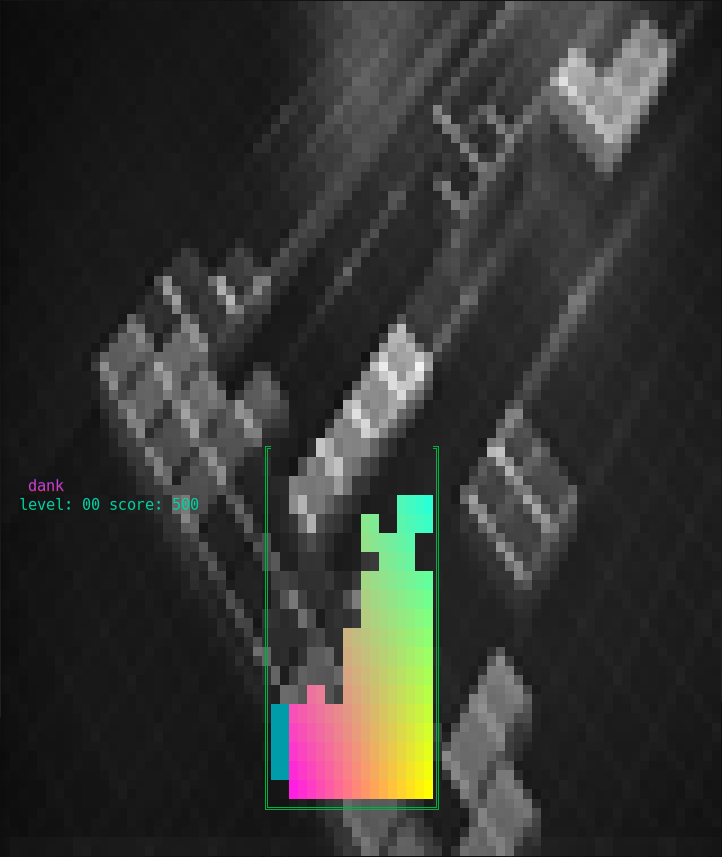
\includegraphics[width=1\linewidth]{media/tetris-prescore.png}
    \caption{Tetris---primed to score.}
  \end{minipage}\hfill
  \begin{minipage}{0.45\textwidth}
    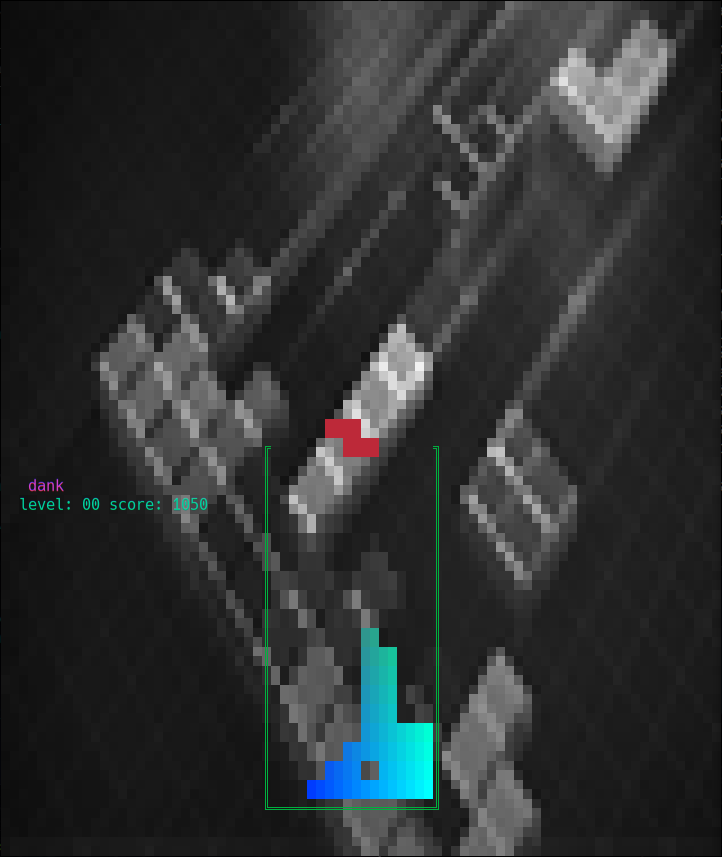
\includegraphics[width=1\linewidth]{media/tetris-postscore.png}
    \caption{Tetris---boom!}
  \end{minipage}
\end{figure}

\begin{figure}
  \centering
  \begin{minipage}{0.45\textwidth}
    \inputminted[]{C}{code-tetris/moveleft.h}
    \caption{\texttt{Tetris::MoveLeft()}.}
  \end{minipage}\hfill
  \begin{minipage}{0.45\textwidth}
    \inputminted[]{C}{code-tetris/moveright.h}
    \caption{\texttt{Tetris::MoveRight()}.}
  \end{minipage}
  \label{list:tetris-move}
\end{figure}

\begin{listing}[!htb]
\inputminted[]{C}{code-tetris/rotate.h}
\caption{\texttt{Tetris::RotateCcw()} and \texttt{Tetris::RotateCw()}.}
\label{list:tetris-rotate}
\end{listing}

\begin{listing}[!htb]
\inputminted[]{C}{code-tetris/main.h}
\caption[]{Tetris \texttt{main()}.}
\label{list:tetris-main}
\end{listing}

Our \texttt{main()} is quite minimal. A \texttt{Tetris} instance is
constructed, initializting the game board and providing necessary state (score,
level, etc.). \texttt{Tetris::Ticker()} is launched as a {\CC}11 thread. We
then loop on input until either the game is over or the user presses 'q'.
Finally, we \texttt{join()} the \texttt{Ticker()} thread, and shut down
Notcurses. We accept function keys or vi keys for movement. 'z' and 'x' rotate
counterclockwise and clockwise respectively. Ctrl+L refreshes the screen to
round out our UI.
